\documentclass{article}
\usepackage[utf8]{inputenc}
\usepackage{amsmath}
\usepackage[a4paper, margin=1in]{geometry}
\usepackage[default]{raleway}
\usepackage{graphicx}
\usepackage{listings}
\usepackage{xcolor}

% Paramètres d'affichage du code
\lstset{
    basicstyle=\ttfamily\footnotesize,
    backgroundcolor=\color{gray!10},
    frame=single,
    breaklines=true,
    keywordstyle=\color{blue}\bfseries,
    commentstyle=\color{green!60!black},
    stringstyle=\color{red!70!black},
    numbers=left,
    numberstyle=\tiny\color{gray},
    stepnumber=1,
    numbersep=10pt,
    showspaces=false,
    showstringspaces=false,
    tabsize=4,
    captionpos=b
}

\begin{document}

\begin{minipage}{0.5\textwidth}
  \centering
  \Large \textbf{Compte-Rendu UC2-MRA} \\
  \vspace{0.5cm}
  \large \textbf{Nom :} TESSON \\
  \textbf{Prénom :} Paul \\
  \textbf{Numéro étudiant :} 20210145
\end{minipage}
\hfill
\begin{minipage}{0.45\textwidth}
  \centering
  
\includegraphics[width=0.8\linewidth]{Logo_ENIB_2012.png}
\end{minipage}

\section*{Introduction}
Ce document présente une évaluation du contrôleur de Braitenberg appliqué à un robot Pioneer dans un environnement simulé sous \textbf{CoppeliaSim} (API \textbf{V-REP}). L'objectif est d'analyser les impacts des paramètres, notamment les poids de la matrice de commande réflexive, sur le comportement du robot, en explorant les limites du modèle.

\section*{Description de la Simulation}
Le robot à roues différentielles est équipé de 16 capteurs ultrasoniques. Ces capteurs influencent directement les moteurs gauche et droit via une matrice de poids définissant les réactions du robot aux obstacles.

\subsection*{Configuration Initiale}
La simulation est configurée avec les paramètres suivants : connexion à un serveur local, chargement d'une scène et initialisation des objets (robot, capteurs, moteurs).

\begin{lstlisting}[language=Python, caption=Connexion et configuration de la simulation]
ip = '127.0.0.1'
port = 19997
scene = './Pioneer_murs.ttt'

print('Program started')
vrep.simxFinish(-1)
client_id = vrep.simxStart(ip, port, True, True, 5000, 5)
if client_id != -1:
    print('Connected to remote API server')
    vrep.simxLoadScene(client_id, scene, 1, vrep.simx_opmode_oneshot_wait)
    res, pioneer = vrep.simxGetObjectHandle(client_id, 'Pioneer_p3dx', vrep.simx_opmode_oneshot_wait)
    res, left_motor = vrep.simxGetObjectHandle(client_id, 'Pioneer_p3dx_leftMotor', vrep.simx_opmode_oneshot_wait)
    res, right_motor = vrep.simxGetObjectHandle(client_id, 'Pioneer_p3dx_rightMotor', vrep.simx_opmode_oneshot_wait)
\end{lstlisting}

\section*{Contrôleur de Braitenberg}
La logique de Braitenberg repose sur une matrice de poids appliquée à chaque capteur pour influencer les vitesses des moteurs. Les poids peuvent être ajustés pour modifier la réaction du robot.

\subsection*{Structure de la Matrice de Poids}
Voici un exemple de matrice utilisée dans la simulation :

\begin{itemize}
    \item \textbf{Poids gauche :} [-0.2, -0.4, ..., -1.6, 0.0, ...]
    \item \textbf{Poids droit :} [-1.6, -1.4, ..., -0.2, 0.0, ...]
\end{itemize}

Les capteurs proches de l'avant ont des poids plus élevés, influençant fortement la vitesse pour éviter les obstacles.

\subsection*{Logique de Commande}
Le code suivant illustre comment les capteurs influencent les moteurs :

\begin{lstlisting}[language=Python, caption=Calcul des vitesses des moteurs]
for i in range(16):
    res, detectionState, detectedPoint, _, _ = vrep.simxReadProximitySensor(client_id, int(sensor_handles[i]), vrep.simx_opmode_buffer)
    if detectionState:
        distToObject = math.sqrt(sum(d ** 2 for d in detectedPoint))
        if distToObject < noDetectionDist:
            detect[i] = 1 - ((distToObject - maxDetectionDist) / (noDetectionDist - maxDetectionDist))
    else:
        detect[i] = 0

vLeft = v0 + sum(braitenbergL[i] * detect[i] for i in range(16))
vRight = v0 + sum(braitenbergR[i] * detect[i] for i in range(16))
\end{lstlisting}

\section*{Analyse des Résultats}

Différentes configurations de poids ont été testées pour évaluer leurs effets sur le comportement du robot. Voici les observations principales :

\subsection*{Effets des Poids}
\begin{itemize}
    \item \textbf{Poids frontaux augmentés :} Comportement de recul accentué.
    \item \textbf{Poids latéraux augmentés :} Virages plus serrés vers l'opposé.
    \item \textbf{Poids équilibrés :} Déplacement stable et prévisible.
\end{itemize}

\begin{figure}[h!]
    \centering
    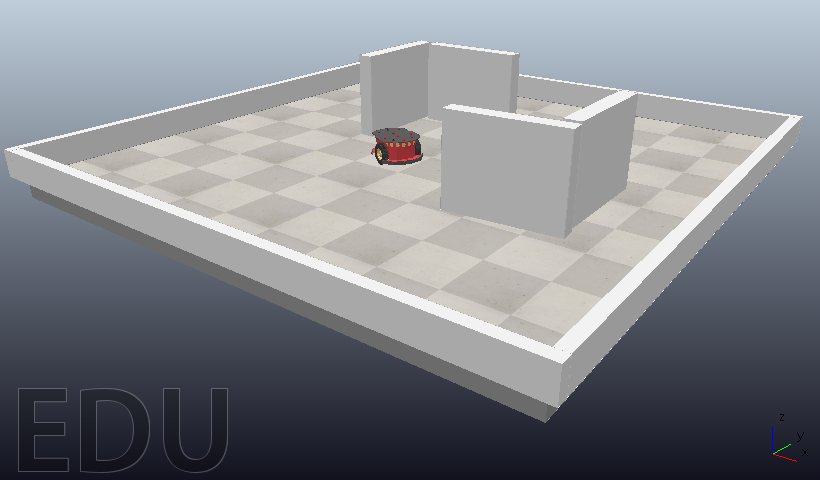
\includegraphics[width=0.5\linewidth]{image_pionneer.PNG}
    \caption{Trajectoire du robot avec différentes matrices de poids.}
    \label{fig:trajectory}
\end{figure}

\subsection*{Limitations et Améliorations}
\begin{itemize}
    \item \textbf{Limite :} Réactions parfois trop sensibles à des obstacles proches.
    \item \textbf{Amélioration :} Ajouter un facteur d'inertie pour lisser les mouvements.
\end{itemize}

\section*{Conclusion}
Les tests montrent que le contrôleur de Braitenberg est efficace pour l'évitement d'obstacles. La modification des poids de la matrice de commande permet de régler finement le comportement du robot. Cette étude met en évidence l'importance de l'ajustement des paramètres pour optimiser la navigation autonome.

\newpage
\appendix
\section*{Annexe : Code Source Complet}

\lstinputlisting[language=Python, caption=Code source complet pour la simulation, label=code:simulation]{control_Pioneer_avec_capteur-IR.py}

\end{document}
